\documentclass[12pt]{article}

\usepackage{booktabs}
\usepackage{tabularx}
\usepackage{hyperref}
\usepackage{graphicx}
\usepackage[a4paper, margin=0.75in]{geometry}
\usepackage{subcaption}
\usepackage{float}
\usepackage{amssymb}
\usepackage[table]{xcolor}
\usepackage{enumitem}
\usepackage{pgfplots}
\pgfplotsset{compat=1.18}
\usepackage{tikz}


\hypersetup{
    colorlinks=true,       % false: boxed links; true: colored links
    linkcolor=red,          % color of internal links (change box color with linkbordercolor)
    citecolor=green,        % color of links to bibliography
    filecolor=magenta,      % color of file links
    urlcolor=cyan           % color of external links
}

\title{Usability Report\\\progname}

\author{\authname}

\date{}

\input{../../Comments}
\input{../../Common}

\begin{document}

\maketitle
\thispagestyle{empty}

~\newpage

\pagenumbering{arabic}

\begin{table}[hp]
\caption{Revision History} \label{TblRevisionHistory}
\begin{tabularx}{\textwidth}{llX}
\toprule
\textbf{Date} & \textbf{Developer(s)} & \textbf{Change}\\
\midrule
04-06-2026 & Virochaan Ravichandran Gowri & Usability Report Final Version\\

... & ... & ...\\
\bottomrule
\end{tabularx}
\end{table}

~\newpage

\tableofcontents

~\newpage

\pagenumbering{arabic}
\section{Introduction}
\subsection{Purpose of the Report}
This report documents the usability testing process and outcomes for the MES Event Management System as a complete product. The purpose is to evaluate how effectively target users can complete core tasks across the platform. There was heavy focus on key end-to-end workflows as well as common practices and usecases. The report captures observed user behavior, friction points, and success rates to determine whether the current design supports clear navigation, understandable interaction patterns, and efficient task completion.

In addition to reporting test outcomes, this document provides evidence-based recommendations for improving the user experience before final release. Findings from this report are intended to guide design refinements and to provide a high importance implementation changes and support traceability between identified usability issues and project decisions in subsequent revisions.
\subsection{Goals of Testing}
The goals of usability testing are to validate that the MES Event Management System is intuitive, accessible, and reliable for its primary stakeholders, and to identify improvements that have the highest impact on user success.

The specific goals are:
\begin{itemize}
    \item Verify that users can complete end-to-end workflows with minimal guidance.
    \item Assess the clarity and consistency of the interface across major surfaces of the project, including the user web portal and the admin portal.
    \item Measure usability indicators such as task completion rate, time on task, error frequency, and user-reported confidence/satisfaction.
    \item Identify interface elements that cause confusion, misclicks, or navigation dead ends, and document actionable fixes.
    \item Evaluate whether feedback states are visible and understandable during common and edge-case interactions.
    \item Confirm that the overall interaction flow aligns with project goals for efficiency and easy learnability for new users.
\end{itemize}
\section{Methodology}
\subsection{User Groups}
Usability testing for the MES Event Management System considered a broad set of stakeholder groups who interact with the platform in different ways. We focused on the primary user groups for testing as they would be the main The following user groups were included for task design and evaluation:

\begin{itemize}
    \item General attendees: Primarily students who will be using this app to register and attend events and also answer forms and provide feedback
    \item Administrative users (MES Executives and Event Organizers): These would be the users responsible for managing the platform and organizing event as well as creating forms.
\end{itemize}

In total we had 6 General Attendee users test our system as well as one Administrative User. We decided that all of the testers would work through both admin and user workflows to maximize the feedback we recieved as well as provide us with new and differing perspectives.
\subsubsection{User Profiles}
For this report, user profiles were intentionally broad and representative rather than persona-specific. Participants were assumed to reflect a typical campus and community event audience with the following baseline demographic characteristics. \\
\\
\textbf{General Attendees:}

\begin{itemize}
    \item Age range: primarily young adults aged 18-24.
    \item Technical familiarity: Experienced with simple technology.
    \item Academic Status: Currently attending University.
    \item Device usage: regular use of laptops and smartphones, with both desktop-first and mobile-first behavior represented.
    \item Language and communication: fluent English users with varied preference for concise labels, visual cues, and guided navigation.
    \item Accessibility needs: users with different visual and interaction preferences.
\end{itemize}
\textbf{Administrative Users:}
\begin{itemize}
    \item Age range: primarily young adults aged 18-24
    \item Technical familiarity: Experience with this type of technology. Used similar alternatives such as google forms and other sources to create these forms in the past. Have experience organizing events online.
    \item Academic Status: Can both be attending University and are a part of the MES or have graduated and are still involved with the MES in an advisory capacity.
    \item Device usage: regular use of laptops and smartphones, with both desktop-first and mobile-first behavior represented.
    \item Language and communication: fluent English users with varied preference for concise labels, visual cues, and guided navigation.
    \item Accessibility needs: users with different visual and interaction preferences.
\end{itemize}

\subsection{Testing Environment}
The testing was done within a \textbf{Chrome Web Browser} to a fully deployed version of our platform to simulate the actual way in which users would interact and utilize our platform.

\subsection{Testing Process}
The testing process consisted of 4 main steps. First we administered a pre-test survey to get some general information regarding the users. Then we let the users do some general exploration of the platform asking them to vocalize their thoughts while using it while we observed. We then asked them to do specific end-to-end workflows as we observed them accomplishing them once again asking them to vocalize their thoughts. Finally we administered a post-testing survey gathering their feedback on the platform and areas of improvement.

\begin{figure}[H]
\centering
\setlength{\fboxsep}{8pt}
\fbox{%
\begin{minipage}{0.95\textwidth}
\centering
\textbf{Pre-Test Survey}
\quad$\rightarrow$\quad
\textbf{Guided Exploration}
\quad$\rightarrow$\quad
\textbf{Task-Based Workflows}
\quad$\rightarrow$\quad
\textbf{Post-Test Survey}
\end{minipage}}
\caption{Usability testing process used for the MES platform}
\label{fig:usability-testing-process}
\end{figure}


\subsubsection{Step 1: Pre-Test Survey}
Before interaction with the system, participants completed a short pre-test survey to collect baseline information. This was for us to understand a bit about the tester's background and experience. The pre-test survey used in this study is listed below: \\
\\
\textbf{Pre-Test Survey}
\begin{enumerate}
    \item What is your role for this testing session?
    \begin{itemize}[label=$\circ$]
        \item General attendee
        \item Administrative user (MES executive/event organizer)
    \end{itemize}
    \item What is your age range?
    \begin{itemize}[label=$\circ$]
        \item 18--20
        \item 21--24
        \item 25--34
        \item 35+
    \end{itemize}
     \item Are you a McMaster Student?
    \begin{itemize}[label=$\circ$]
        \item Yes
        \item No
    \end{itemize}
    \item Which device do you use most often?
    \begin{itemize}[label=$\circ$]
        \item Laptop/Desktop
        \item Smartphone
        \item Tablet
    \end{itemize}
    \item Have you previously used tools such as Google Forms, Eventbrite, or similar platforms?
    \begin{itemize}[label=$\circ$]
        \item Yes
        \item No
    \end{itemize}
    \item How confident are you in completing common web tasks (navigation, form completion, and account actions)?
    \begin{itemize}[label=$\circ$]
        \item Low
        \item Medium
        \item High
    \end{itemize}
    \item Do you have any accessibility preferences we should account for during the session?
    \begin{itemize}[label=$\circ$]
        \item No
        \item Larger text
        \item Higher contrast
        \item Keyboard-first interaction
        \item Other (short response)
    \end{itemize}
\end{enumerate}

Responses to this survey were used only to contextualize usability findings and segment observations by user type and experience level.

\subsubsection{Step 2: Guided Exploration}
Participants were then asked to freely explore the platform while thinking aloud. During this stage, moderators observed navigation behavior, first impressions, and areas where labels or layout created uncertainty. This helped identify discoverability and learnability issues before introducing formal tasks. This stage also 

\subsubsection{Step 3: Task-Based Workflow Evaluation}
After exploration, participants completed targeted end-to-end workflows aligned with the primary use-cases of the platform. These workflows were separated so that both attendee-facing and administrative functionality could be evaluated in a realistic context. \textbf{All Testers} worked through the workflows so we could have a wide variety of data and perspectives on the different processes within the platform.

\textbf{General User Workflows}
\begin{itemize}
    \item \textbf{Creating an account:} Users were asked to register a new account and move through the standard account creation flow.
    \item \textbf{Registering for an event, including completion of the payment flow:} Users were asked to browse to an event, begin registration, and complete any required payment steps to evaluate the smoothness of the sign-up process. They were then asked to locate and show the ticket.
    \item \textbf{Completing a survey:} Users were asked to locate and submit a survey so that the team could assess whether form questions, navigation, and submission feedback were clear and intuitive.
\end{itemize}

\textbf{Administrative User Workflows}
\begin{itemize}
    \item \textbf{Creating an event:} Administrative users were asked to create a new event and configure its core information to evaluate the event setup interface.
    \item \textbf{Creating a form:} Administrative users were asked to build a standard 5 question form using all question types.
    \item \textbf{Creating a modular form:} Administrative users were asked to construct a modular form with reusable or organized sections to evaluate whether more advanced form-building functionality remained understandable and manageable.
    \item \textbf{Viewing form analytics:} Administrative users were asked to access analytics for an existing form and to export these form analytics to a csv file.
\end{itemize}
During these workflows, observers recorded task completion, time on task, user hesitation, navigation errors, and points where participants required clarification. This step provided the main evidence for identifying usability issues tied to the system's core functionality.

\subsubsection{Step 4: Post-Test Survey and Debrief}
At the end of each session, participants completed a detailed post-test survey and a short debrief discussion. The survey was divided into common questions for all participants and role-specific questions for the two primary user groups. This structure allowed the team to evaluate both overall usability and workflow-specific concerns.

\textbf{Post-Test Survey Structure}

\textbf{Section A: Overall Experience Questions for All Users}
\begin{enumerate}
    \item Overall, how easy was the platform to use?
    \begin{itemize}[label=$\circ$]
        \item Very difficult
        \item Difficult
        \item Neutral
        \item Easy
        \item Very easy
    \end{itemize}
    \item How clear was the navigation throughout the platform?
    \begin{itemize}[label=$\circ$]
        \item Very unclear
        \item Unclear
        \item Neutral
        \item Clear
        \item Very clear
    \end{itemize}
    \item How confident would you feel using the platform again without assistance?
    \begin{itemize}[label=$\circ$]
        \item Not confident at all
        \item Slightly confident
        \item Moderately confident
        \item Confident
        \item Very confident
    \end{itemize}
    \item How visually clear and readable was the interface?
    \begin{itemize}[label=$\circ$]
        \item Very poor
        \item Poor
        \item Acceptable
        \item Good
        \item Excellent
    \end{itemize}
    \item How useful were the feedback messages shown by the system (for example, success, warning, or error messages)?
    \begin{itemize}[label=$\circ$]
        \item Not useful
        \item Slightly useful
        \item Moderately useful
        \item Useful
        \item Very useful
    \end{itemize}
    \item Did you encounter any point where you were unsure what to do next?
    \begin{itemize}[label=$\circ$]
        \item Yes
        \item No
    \end{itemize}
    \item Which part of the platform felt the most intuitive to use?
    \begin{itemize}[label=$\square$]
        \item Account-related actions
        \item Event browsing or event management
        \item Forms and surveys
        \item Analytics and reporting
        \item Other (short response)
    \end{itemize}
    \item Which part of the platform felt the most confusing or frustrating?
    \begin{itemize}[label=$\circ$]
        \item Navigation
        \item Form completion or form creation
        \item Registration or payment flow
        \item Event setup or management
        \item Analytics or reporting
        \item Other (short response)
    \end{itemize}
    \item What was the single biggest usability issue you experienced?\\
    \underline{\hspace{15cm}}
    \item What improvement would most improve your experience with the platform?\\
    \underline{\hspace{15cm}}
\end{enumerate}

\textbf{Section B: User Portal Questions}
\begin{enumerate}
    \item How easy was it to create a new account?
    \begin{itemize}[label=$\circ$]
        \item Very difficult
        \item Difficult
        \item Neutral
        \item Easy
        \item Very easy
    \end{itemize}
    \item How clear were the fields and instructions during account creation?
    \begin{itemize}[label=$\circ$]
        \item Very unclear
        \item Unclear
        \item Neutral
        \item Clear
        \item Very clear
    \end{itemize}
    \item How easy was it to find and register for an event?
    \begin{itemize}[label=$\circ$]
        \item Very difficult
        \item Difficult
        \item Neutral
        \item Easy
        \item Very easy
    \end{itemize}
    \item How comfortable did you feel during the payment process?
    \begin{itemize}[label=$\circ$]
        \item Very uncomfortable
        \item Uncomfortable
        \item Neutral
        \item Comfortable
        \item Very comfortable
    \end{itemize}
    \item How easy was it to locate your event ticket or registration confirmation after registering?
    \begin{itemize}[label=$\circ$]
        \item Very difficult
        \item Difficult
        \item Neutral
        \item Easy
        \item Very easy
    \end{itemize}
    \item How easy was it to find and complete a survey?
    \begin{itemize}[label=$\circ$]
        \item Very difficult
        \item Difficult
        \item Neutral
        \item Easy
        \item Very easy
    \end{itemize}
    \item Did the survey submission process clearly show that your responses were saved successfully?
    \begin{itemize}[label=$\circ$]
        \item Yes
        \item No
        \item Not sure
    \end{itemize}
    \item What attendee-facing feature did you find most useful?
    \begin{itemize}[label=$\circ$]
        \item Account creation
        \item Event browsing
        \item Event registration
        \item Ticket access
        \item Survey completion
        \item Other (short response)
    \end{itemize}
\end{enumerate}

\textbf{Section C: Admin Portal Questions}
\begin{enumerate}
    \item How easy was it to create and configure a new event?
    \begin{itemize}[label=$\circ$]
        \item Very difficult
        \item Difficult
        \item Neutral
        \item Easy
        \item Very easy
    \end{itemize}
    \item How clear were the event creation fields and setup options?
    \begin{itemize}[label=$\circ$]
        \item Very unclear
        \item Unclear
        \item Neutral
        \item Clear
        \item Very clear
    \end{itemize}
    \item How easy was it to create a standard form?
    \begin{itemize}[label=$\circ$]
        \item Very difficult
        \item Difficult
        \item Neutral
        \item Easy
        \item Very easy
    \end{itemize}
    \item How understandable was the modular form creation workflow?
    \begin{itemize}[label=$\circ$]
        \item Very confusing
        \item Confusing
        \item Neutral
        \item Understandable
        \item Very understandable
    \end{itemize}
    \item How easy was it to manage question types, sections, and form structure?
    \begin{itemize}[label=$\circ$]
        \item Very difficult
        \item Difficult
        \item Neutral
        \item Easy
        \item Very easy
    \end{itemize}
    \item How easy was it to locate and understand form analytics?
    \begin{itemize}[label=$\circ$]
        \item Very difficult
        \item Difficult
        \item Neutral
        \item Easy
        \item Very easy
    \end{itemize}
    \item How useful and understandable was the exported analytics data?
    \begin{itemize}[label=$\circ$]
        \item Not useful
        \item Slightly useful
        \item Moderately useful
        \item Useful
        \item Very useful
    \end{itemize}
    \item Which administrative workflow needs the most improvement?
    \begin{itemize}[label=$\circ$]
        \item Event creation
        \item Standard form creation
        \item Modular form creation
        \item Analytics viewing/export
        \item Other (short response)
    \end{itemize}
\end{enumerate}

\textbf{Section D: Open-Ended Feedback Questions}
\begin{enumerate}
    \item Please describe your overall impression of the MES Event Management System. What stood out most to you, whether positively or negatively? \\
    \underline{\hspace{15cm}}
    \item If you were to redesign one aspect of the platform based on your experience today, what would it be and why? \\
    \underline{\hspace{15cm}}
    \item How would you compare this platform to other similar event management or registration systems you have used? What does this system do better or worse? \\
    \underline{\hspace{15cm}}
    \item What would make you more likely to recommend this platform to a friend or colleague? \\
    \underline{\hspace{15cm}}
    \item From an attendee's perspective, what is the most important feature the platform should have? \\
    \underline{\hspace{15cm}}
    \item What workflow or feature would save you the most time when managing events and forms? \\
    \underline{\hspace{15cm}}
    \item What capabilities do you wish the platform had that are currently missing? \\
    \underline{\hspace{15cm}}
\end{enumerate}

Responses from this survey, including both quantitative ratings and qualitative open-ended feedback, were combined with observation notes and task performance metrics to prioritize usability issues and recommend improvements for future iterations of the platform.


\section{Findings}
\subsection{Testing Feedback}

\subsubsection{Quantitative Results}

The post-test survey (Step 4, Section A) asked all 7 participants to rate five overall experience dimensions on a 5-point scale. Scores below reflect averages across all participants, where 1 = Very Difficult / Very Poor / Not Confident / Not Useful and 5 = Very Easy / Excellent / Very Confident / Very Useful.

\begin{figure}[H]
\centering
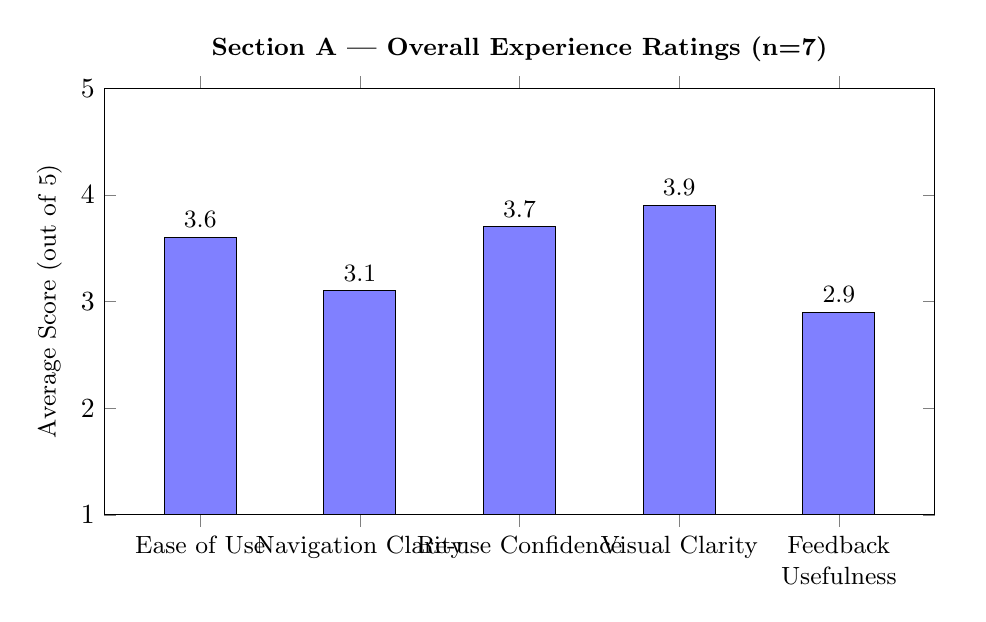
\begin{tikzpicture}
\begin{axis}[
    ybar,
    bar width=26pt,
    width=\textwidth,
    height=7cm,
    symbolic x coords={Ease of Use, Navigation Clarity, Re-use Confidence, Visual Clarity, Feedback Usefulness},
    xtick=data,
    x tick label style={font=\small, align=center, text width=2.8cm},
    ymin=1, ymax=5,
    ytick={1,2,3,4,5},
    ylabel={Average Score (out of 5)},
    ylabel style={font=\small},
    nodes near coords,
    nodes near coords align={vertical},
    every node near coord/.append style={font=\small},
    enlarge x limits=0.15,
    title={Section A --- Overall Experience Ratings (n=7)},
    title style={font=\small\bfseries},
]
\addplot[fill=blue!50] coordinates {
    (Ease of Use,         3.6)
    (Navigation Clarity,  3.1)
    (Re-use Confidence,   3.7)
    (Visual Clarity,      3.9)
    (Feedback Usefulness, 2.9)
};
\end{axis}
\end{tikzpicture}
\caption{Average post-test survey ratings for Section A overall experience questions}
\label{fig:overall-ratings}
\end{figure}

Visual Clarity was the highest-rated dimension (3.9), indicating that participants found the general appearance of the platform acceptable. Navigation Clarity (3.1) and Feedback Usefulness (2.9) were the weakest dimensions, both falling below neutral. These scores directly reflect confusion observed during Step 2 free exploration, where participants frequently paused at tab transitions and reported uncertainty about whether actions had been registered by the system.

Section A also asked whether participants encountered a point where they were unsure what to do next. 5 of 7 participants answered Yes. Asked to identify the most confusing or frustrating area (Section A, Q8), responses were distributed as follows:

\begin{figure}[H]
\centering
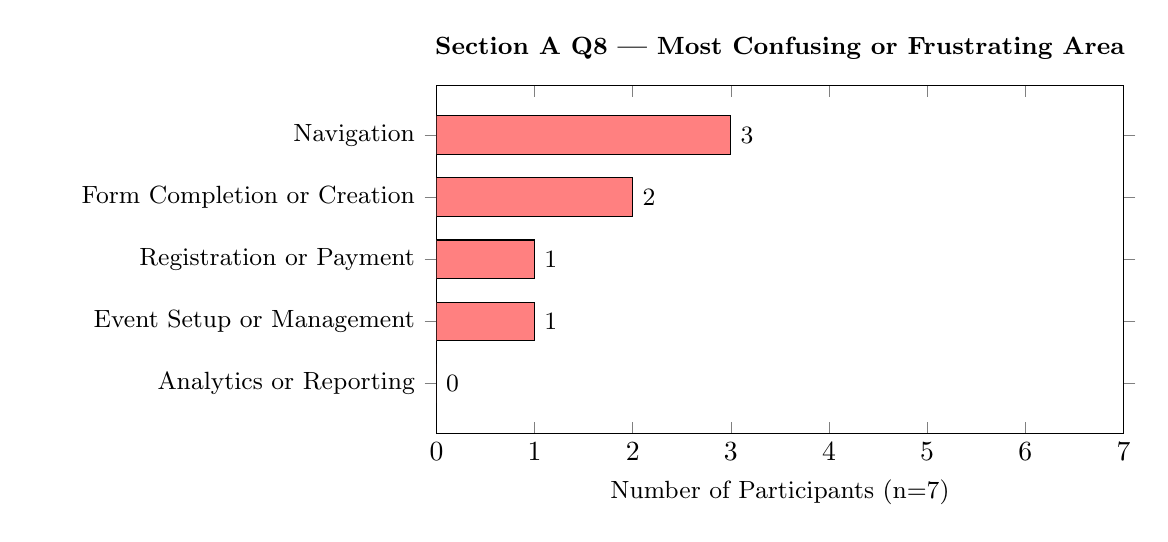
\begin{tikzpicture}
\begin{axis}[
    xbar,
    bar width=14pt,
    width=0.85\textwidth,
    height=6cm,
    symbolic y coords={Analytics or Reporting, Event Setup or Management, Registration or Payment, Form Completion or Creation, Navigation},
    ytick=data,
    y tick label style={font=\small, align=right, text width=4.8cm},
    xmin=0, xmax=7,
    xtick={0,1,2,3,4,5,6,7},
    xlabel={Number of Participants (n=7)},
    xlabel style={font=\small},
    nodes near coords,
    nodes near coords align={horizontal},
    every node near coord/.append style={font=\small},
    enlarge y limits=0.2,
    title={Section A Q8 --- Most Confusing or Frustrating Area},
    title style={font=\small\bfseries},
]
\addplot[fill=red!50] coordinates {(0,Analytics or Reporting) (1,Event Setup or Management) (1,Registration or Payment) (2,Form Completion or Creation) (3,Navigation)};
\end{axis}
\end{tikzpicture}
\caption{Participant responses to Section A Q8: most confusing or frustrating platform area}
\label{fig:frustration-areas}
\end{figure}

Navigation was selected by 3 of 7 participants as the most frustrating area, consistent with the low Navigation Clarity score and the tab routing issues observed repeatedly during Step 3 task workflows.

The user portal workflow questions (Section B) asked participants to rate specific attendee-facing tasks:

\begin{figure}[H]
\centering
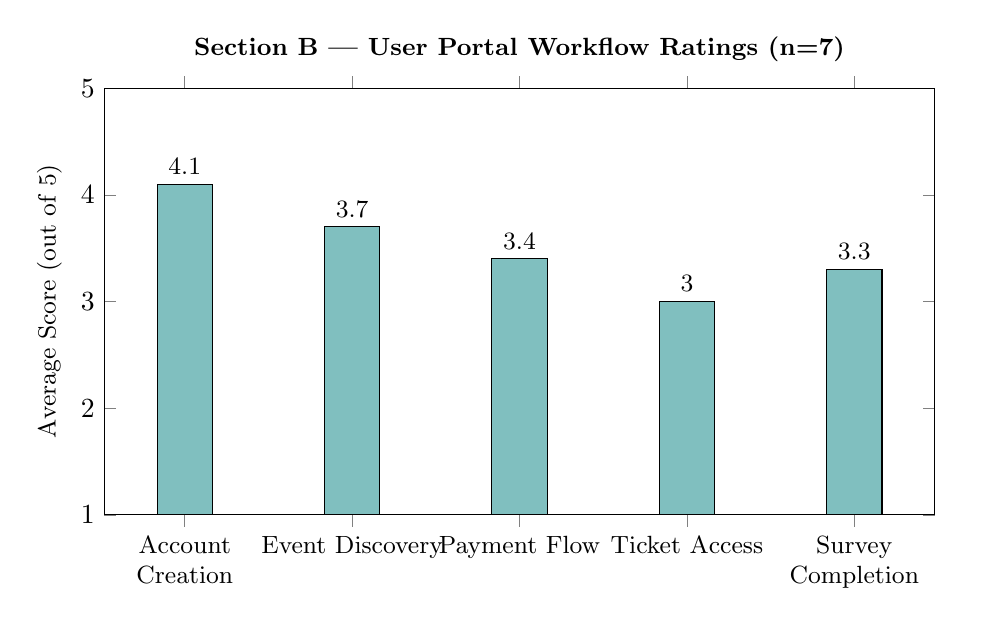
\begin{tikzpicture}
\begin{axis}[
    ybar,
    bar width=20pt,
    width=\textwidth,
    height=7cm,
    symbolic x coords={Account Creation, Event Discovery, Payment Flow, Ticket Access, Survey Completion},
    xtick=data,
    x tick label style={font=\small, align=center, text width=2.4cm},
    ymin=1, ymax=5,
    ytick={1,2,3,4,5},
    ylabel={Average Score (out of 5)},
    ylabel style={font=\small},
    nodes near coords,
    nodes near coords align={vertical},
    every node near coord/.append style={font=\small},
    enlarge x limits=0.12,
    title={Section B --- User Portal Workflow Ratings (n=7)},
    title style={font=\small\bfseries},
]
\addplot[fill=teal!50] coordinates {
    (Account Creation,  4.1)
    (Event Discovery,   3.7)
    (Payment Flow,      3.4)
    (Ticket Access,     3.0)
    (Survey Completion, 3.3)
};
\end{axis}
\end{tikzpicture}
\caption{Average post-test ratings for Section B user portal workflow questions}
\label{fig:user-portal-ratings}
\end{figure}

Account creation was the smoothest workflow (4.1). Ticket access scored lowest (3.0), reflecting the Step 3 observation that multiple participants could not immediately locate their registration confirmation after completing the event registration task. Section B Q7 asked whether the survey submission process clearly showed that responses were saved: 4 of 7 participants answered No or Not Sure, corroborating the low Survey Completion score.

The admin portal questions (Section C) covered four administrative workflows:

\begin{figure}[H]
\centering
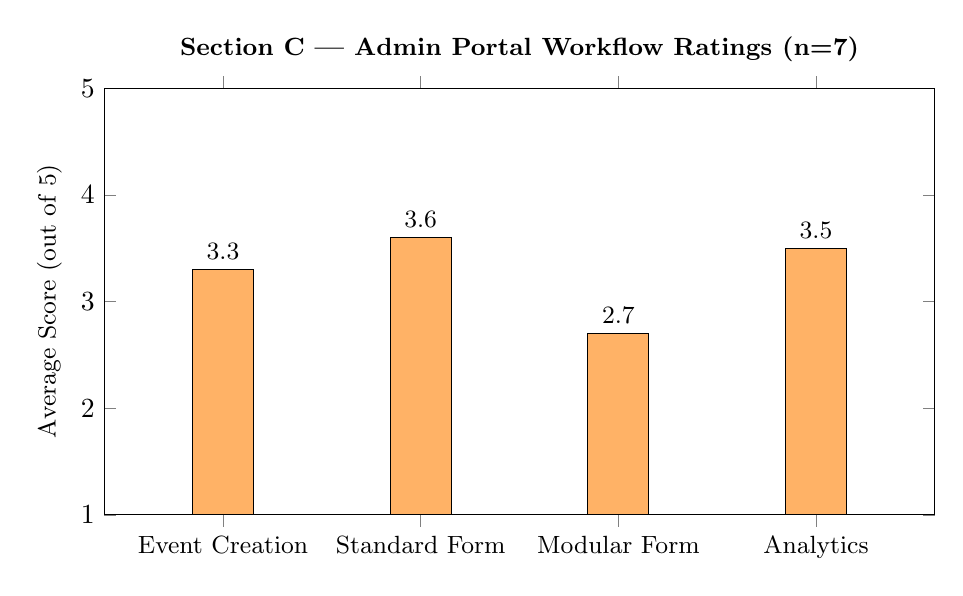
\begin{tikzpicture}
\begin{axis}[
    ybar,
    bar width=22pt,
    width=\textwidth,
    height=7cm,
    symbolic x coords={Event Creation, Standard Form, Modular Form, Analytics},
    xtick=data,
    x tick label style={font=\small, align=center, text width=2.4cm},
    ymin=1, ymax=5,
    ytick={1,2,3,4,5},
    ylabel={Average Score (out of 5)},
    ylabel style={font=\small},
    nodes near coords,
    nodes near coords align={vertical},
    every node near coord/.append style={font=\small},
    enlarge x limits=0.2,
    title={Section C --- Admin Portal Workflow Ratings (n=7)},
    title style={font=\small\bfseries},
]
\addplot[fill=orange!60] coordinates {
    (Event Creation, 3.3)
    (Standard Form,  3.6)
    (Modular Form,   2.7)
    (Analytics,      3.5)
};
\end{axis}
\end{tikzpicture}
\caption{Average post-test ratings for Section C admin portal workflow questions}
\label{fig:admin-portal-ratings}
\end{figure}

Modular form creation was the lowest-rated admin workflow (2.7). During the Step 3 modular form creation task, observers noted that all participants required prompting at least once to proceed, and several reached an indeterminate state without realising it. Event creation also scored below the midpoint for field clarity (Section C Q2), driven by confusion around the visibility toggle and the unlock date field observed during the Step 3 event creation task.

\subsubsection{Component Specific Feedback}

The following observations are drawn from think-aloud commentary recorded during Step 2 (Guided Exploration) and Step 3 (Task-Based Workflows), and from open-ended responses in Section D of the post-test survey.

\textbf{User Portal}
\begin{itemize}
    \item \textit{Alerts and native components:} During Step 2 free exploration, multiple participants reacted visibly to the browser-native alert dialogs that appeared on form submission, commenting that they looked out of place. The native OS select dropdowns were similarly flagged as inconsistent with the rest of the interface. In Section D, two participants noted the visual inconsistency of these components when asked to describe their overall impression of the platform.

    \item \textit{Tab navigation and routing:} During the Step 3 survey completion task, participants who navigated back from a submitted form were returned to the Overview tab rather than the Surveys tab. Several participants expressed confusion, re-browsed to the Surveys tab, and then attempted to determine whether their submission had been recorded. This was one of the most frequently observed hesitation points across Step 3 sessions. Navigation was selected by 3 of 7 participants as the most frustrating area in Section A Q8.

    \item \textit{Form save state and edit flow:} During the Step 3 survey completion task, participants who saved a partial response and reloaded the page found no responses persisted. When subsequently asked to edit a prior submission, the form opened blank rather than pre-filled with previous answers. Participants expressed uncertainty about whether the save function was working at all. Section B Q7 confirmed this: 4 of 7 participants indicated the submission process did not clearly confirm that responses had been saved.

    \item \textit{Event registration --- repeated user fields:} During the Step 3 event registration task, participants were presented with fields for first name, last name, and email despite being logged in. This was commented on unprompted by multiple participants during think-aloud. In Section D, this was cited by two participants as the improvement that would most benefit their experience.

    \item \textit{Post-registration confirmation:} After completing the Step 3 event registration task, participants were asked to locate their ticket. Several attempted to register a second time because the event page showed no visible change after registration. This directly contributed to the lower Ticket Access score (3.0) in Section B and was cited in Section A Q9 as the single biggest usability issue by two participants.

    \item \textit{Featured Events --- View Details routing:} During Step 2 free exploration, participants clicked ``View Details'' on the Overview tab expecting to land on the specific event page. When they were taken to the Events tab instead, several participants initially believed the link had not worked. This was noted in Section D open-ended responses as a confusing first impression.

    \item \textit{Form card timestamps:} During Step 2, participants browsing the form list questioned what the date displayed on each card represented. Think-aloud commentary included uncertainty about whether it reflected when the form was created or last updated. No participant was able to determine this from the UI alone.
\end{itemize}

\textbf{Admin Portal}
\begin{itemize}
    \item \textit{Visibility toggle and unlock date:} During the Step 3 event creation task, all participants paused when reaching the visibility toggle. The toggle's design led participants to interpret ``private'' as an inactive or disabled state. The adjacent ``Set Date'' label was not understood to be connected to an unlock date mechanism without prompting. In Section C Q2, field clarity for event creation scored below neutral, and this section was the primary contributor to that result.

    \item \textit{Unlock date validation:} During Step 3, participants who entered an invalid date into the unlock date field and saved observed the field clear silently. No error message appeared. Participants expressed uncertainty about whether their input had been accepted or discarded, and in some cases re-entered the date without realising it had already been cleared.

    \item \textit{Admin event page routing:} During Step 3 administrative workflows, navigating to an event from the admin events list failed to load the event content in some cases. Participants who encountered this attempted refreshing and re-clicking before concluding the page was broken. This was observed during task execution and noted in Section D open-ended responses.

    \item \textit{Duplicate registrations:} During Step 3, the absence of post-registration confirmation on the event page led participants to register for the same event more than once. This was flagged by the administrative tester as a data integrity concern when reviewing the registrations table.

    \item \textit{Registrations table layout:} During the Step 3 admin workflow, participants reviewing the registrations table commented that combining first and last name into a single column made it harder to scan. This was raised in the Section D open-ended question about what workflow or feature would save the most time.

    \item \textit{``Instance'' label and event status:} During Step 2 exploration of the admin portal, no general-user participant understood what ``Instance'' referred to. The ``Scheduled'' event status was also questioned during Step 3, with participants unsure whether it updated automatically or required manual changes.

    \item \textit{Non-functional eye icon:} During Step 2 free exploration, participants noticed the eye icon in the admin interface and attempted to use it, expecting a preview. When it produced no result, participants were unsure whether they had missed something or whether the feature was incomplete.

    \item \textit{Form title and description editing:} During Step 3, participants who wanted to correct a form title after creation could not find a clear path to do so. This was raised in Section D open-ended responses when participants were asked what they would redesign.

    \item \textit{Form card height inconsistency:} Observed during Step 2 exploration of the admin form list. Cards without descriptions rendered noticeably shorter than those with descriptions, producing a visually uneven grid. Participants did not raise this verbally but it was recorded as an observer note.
\end{itemize}

\textbf{Form Builder}
\begin{itemize}
    \item \textit{Bulk option entry:} During the Step 3 standard form creation task, participants building dropdown or multiple-choice questions with many options expressed frustration at having to click ``Add Choice'' individually for each entry. In Section D, this was raised in response to the question about what capabilities they wished the platform had, with explicit comparison to Google Forms' paste-to-populate behaviour.

    \item \textit{Add Choice focus and Enter key:} Observed during Step 3 form creation tasks. After clicking ``Add Choice,'' participants had to click the new input row before typing. Pressing Enter in a choice field did not create the next row. Both behaviours were expected by participants based on prior experience with Google Forms.

    \item \textit{Multi-select ``Required'' label:} During Step 3, participants configuring a multi-select question interpreted the ``Required'' label on the selection limit field as a question-level required marker. This led to incorrect configuration in several sessions and was noted in Section C Q5 responses regarding ease of managing question types.

    \item \textit{Red border on question selection:} Observed during Step 3 form creation. Selecting a question in the builder triggered a red border, which every participant interpreted as a validation error. Participants paused and attempted to identify what they had done wrong before realising the border indicated selection.
\end{itemize}

\subsubsection{Observations and General Impressions}

Across all seven sessions, participants responded positively to the visual design of the platform during Step 2 exploration, frequently describing it as clean and well-structured. This is consistent with the Visual Clarity score of 3.9 from Section A of the post-test survey, which was the highest-rated dimension overall.

Functional clarity was a recurring concern. Think-aloud commentary during Steps 2 and 3 showed that participants frequently paused at transition points between sections --- particularly when returning from a completed form or event registration --- and were uncertain whether their prior action had been recorded. This pattern is reflected in the low Feedback Usefulness score (2.9) from Section A and in the Section B Q7 result, where 4 of 7 participants indicated the submission process did not clearly confirm their responses had been saved.

Participants carried strong expectations from prior experience with Google Forms, Eventbrite, and similar platforms, as indicated by pre-test survey responses confirming all participants had used such tools before. When the MES platform deviated from familiar patterns --- such as not auto-populating known user fields, not restoring draft responses, or not routing back to the correct tab after navigation --- participants noticed the deviation immediately and commented on it during think-aloud.

All participants successfully completed the account creation and event browsing tasks in Step 3. Task completion was less consistent for ticket access, the modular form creation workflow, and the event visibility and unlock date configuration task. In these cases, participants either required direct prompting to proceed or reached an incorrect end state without realising it. These outcomes are reflected in the lower post-test scores for Ticket Access (Section B, 3.0) and Modular Form creation (Section C, 2.7).

\subsection{Usability Issues}

\subsubsection{Major Issues}

\begin{itemize}
    \item \textbf{No post-registration confirmation on the event page.} Observed in every Step 3 event registration session. After completing registration, the event page showed no visible change. Multiple participants attempted to register a second time. This produced the lowest user portal score for Ticket Access (Section B, 3.0) and was cited as the biggest usability issue by two participants in Section A Q9. This issue also surfaced in the admin portal as duplicate registration records.

    \item \textbf{Tab state not preserved on navigation.} Observed consistently during Step 3 survey completion and event registration tasks. Returning from a form or event page dropped participants back to the Overview tab regardless of origin. Navigation was selected as the most frustrating area by 3 of 7 participants in Section A Q8, and Navigation Clarity received the second-lowest overall rating (3.1) in Section A.

    \item \textbf{Draft responses not persisted; edit view does not pre-fill prior answers.} Observed during Step 3 survey completion. Saving a partial response and reloading produced a blank form. Opening a prior submission for editing also produced a blank form. Confirmed by Section B Q7: 4 of 7 participants indicated the platform did not clearly show that responses had been saved. Feedback Usefulness scored 2.9 in Section A, the lowest overall dimension.

    \item \textbf{Known user fields not pre-populated during event registration.} Observed during Step 3 event registration. Authenticated participants were asked to re-enter their name and email. Multiple participants commented on this unprompted during think-aloud. Two participants cited this in Section D as the single improvement that would most benefit their experience.

    \item \textbf{Visibility toggle design and unlock date field are unclear.} Observed during Step 3 event creation. The toggle design caused participants to misread the state semantics, and the ``Set Date'' label was not understood as controlling an unlock date. Event creation field clarity scored below neutral in Section C Q2. The unlock date silently discarding invalid input further compounded the issue.

    \item \textbf{Modular form creation workflow is not sufficiently clear.} Observed during Step 3. All participants required at least one prompt during the modular form creation task, and some reached an indeterminate state without recognising it. Modular Form creation received the lowest admin workflow rating (Section C, 2.7). Section C Q8 identified modular form creation as the administrative workflow most in need of improvement.

    \item \textbf{Browser-native alerts and dropdowns break interface consistency.} Observed during Step 2 free exploration by multiple participants without prompting. Cited in Section D open-ended responses when participants described their overall impression of the platform. Contributes to the gap between the high Visual Clarity score and the lower overall Ease of Use rating.
\end{itemize}

\subsubsection{Minor Issues}

\begin{itemize}
    \item \textbf{``View Details'' on Featured Events routes to the Events tab, not the specific event.} Observed during Step 2 free exploration. Participants expected to land on the individual event page and interpreted the misdirection as the link not working. Raised in Section D open-ended responses as a confusing first impression.

    \item \textbf{Form card timestamps are ambiguous.} Observed during Step 2 exploration of the form list. Participants could not determine from the UI whether the date represented creation, last edit, or last submission.

    \item \textbf{``Add Choice'' does not auto-focus the new row, and Enter does not create the next option.} Observed during Step 3 form creation tasks. Both behaviours were expected based on participant familiarity with Google Forms, confirmed in pre-test survey responses. Raised explicitly in Section D when participants described missing capabilities.

    \item \textbf{Paste-to-populate not supported for bulk option entry.} Observed during Step 3 form creation. Participants building long option lists expressed frustration. Explicitly cited in Section D responses to the question about what capabilities the platform was missing, with direct comparison to Google Forms.

    \item \textbf{Multi-select ``Required'' label is misleading.} Observed during Step 3 form creation. Participants consistently misread the label as a question-level required marker. Contributed to the below-neutral rating for managing question types in Section C Q5.

    \item \textbf{Red border on question selection resembles a validation error.} Observed during Step 3 form creation. Every participant paused and attempted to identify an error before realising the border indicated selection state.

    \item \textbf{Admin registrations table combines first and last name into one column.} Observed during Step 3 administrative workflows. Raised in Section D open-ended responses when participants were asked what would save them the most time.

    \item \textbf{``Instance'' label and event status are not understood.} Observed during Step 2 admin portal exploration. No general-user participant understood ``Instance'' without prompting. Event status ambiguity was raised during Step 3 event creation.

    \item \textbf{Non-functional eye icon in the admin interface.} Observed during Step 2 free exploration. Participants attempted to use it and were confused by the lack of response.

    \item \textbf{Form cards without descriptions render at inconsistent heights.} Recorded as an observer note during Step 2 exploration of the admin form list.

    \item \textbf{Payment option remains visible to users who have already paid.} Observed during Step 3 event registration and flagged during the post-test debrief discussion.

    \item \textbf{No mechanism to mark a registrant as Attended.} Raised by the administrative tester during Step 3 and in the Section D open-ended response about missing capabilities.
\end{itemize}


\section{Recommendations}
\subsection{High Priority Improvements}
These are the fixes that we will be focusing on to ensure that our platform will be highly useable and ensure a good quality product.
\begin{itemize}
    \item Replace browser-default components such as alerts and form components with custom components to ensure cohesive styling and more professionel platform design.
    \item Implement URL or search-parameter routing for for the user portal so that navigation returns users to the correct tab. Fix navigation routing on the admin portal as well.
    \item Display previously submitted form responses in a read-only format when viewing a submission.
    \item Pre-populate the edit submission view with the user's previously submitted answers and persist response across the page reloads.
    \item Auto-populate known user fields (first name, last name, email) during event registration.
    \item Link 'View Details' on Featured Events directly to the specific event page rather than the Events tab.
    \item Show a visible confirmation state on the event page after a user registers.
    \item Display the timestamp of the latest edit or submission on form cards rather than the creation date.
    \item Redesign Form Builder for better clarity to understand button use cases as well as general workflow.
    \item Clarify the relationship between visibility state and unlock date, and consider consolidating into three explicit states: Private, Publish After Date, and Public. Lock editing of components on published forms to account for data integrity.
    \item Support paste-to-populate for bulk option entry in the form builder, splitting newline-separated values into individual choices.
    \item Support pressing Enter to add the next option when building form choices. Auto-focus the newly created row when adding a choice in the form builder.
\end{itemize}
\subsection{Low Priority Improvements}
\begin{itemize}
    \item Minor UI improvements for more consistency across components and setions of the platform
    \item Fix the various tables for better consistency and readability
    \item Update the UI on the user portal to be more engaging and modern.
    \item Add a mechanism for admins to update a registrant's status from Registered to Attended manually.
    \item Hide or conditionally disable the payment option for users who have already paid.
\end{itemize}
\subsection{Feedback Not Implemented}
\begin{itemize}
    \item Full resolution of the unlock date and private/public visibility interaction model was deferred pending a dedicated design decision on the intended behaviour.
    \item Redesigning visibility and scheduling as a formal three-state system was documented but deferred to a future iteration.
    \item Automatic triggers for changing between event states was considered but decided to move to a future expansion. 
    \item More detailed insights and automatic pdf report generation was considered but 
\end{itemize}


\end{document}